\documentclass{beamer}

\usepackage[utf8]{inputenc}
\usepackage[brazil]{babel}
\usepackage{graphicx,hyperref,icmc,url}

\usepackage{multirow}

% The title of the presentation:
%  - first a short version which is visible at the bottom of each slide;
%  - second the full title shown on the title slide;
\title[Trabalho de Conclusão de Curso]{Aplicação de deep learning em dispositivos Android}

% Optional: a subtitle to be dispalyed on the title slide
\subtitle{}

% The author(s) of the presentation:
%  - again first a short version to be displayed at the bottom;
%  - next the full list of authors, which may include contact information;
\author[Tiago de Miranda Leite]{
    \Large{Tiago de Miranda Leite} \\ \medskip
    \small{NUSP: 7595289} \\
    \small{\href{mailto:tiago.miranda.leite@usp.br}{\nolinkurl{tiago.miranda.leite@usp.br}}} \\ \bigskip
    \small{Orientador: Prof. Dr. João do Espírito Santo Batista Neto} \\ \bigskip
    \large{Apresentação do Trabalho de Conclusão de Curso}
}

% The institute:
%  - to start the name of the university as displayed on the top of each slide
%    this can be adjusted such that you can also create a Dutch version
%  - next the institute information as displayed on the title slide
\institute[ICMC/USP]{
    Bacharelado em Ciências de Computação \\
    Instituto de Ciências Matemáticas e de Computação -- ICMC \\
    Universidade de São Paulo - USP
}

% Add a date and possibly the name of the event to the slides
%  - again first a short version to be shown at the bottom of each slide
%  - second the full date and event name for the title slide
\date[28/11/2018]{\footnotesize{28 de Novembro de 2018}}

\AtBeginSection[]
{
    \begin{frame}<beamer>{Sumário}
        \tableofcontents[currentsection]
    \end{frame}
}

\begin{document}
    
    \begin{frame}[plain]
        \titlepage
    \end{frame}
    
    \begin{frame}
      \frametitle{Sumário}
      \tableofcontents
    \end{frame}
    
    % Section titles are shown in at the top of the slides with the current section 
    % highlighted. Note that the number of sections determines the size of the top 
    % bar, and hence the university name and logo. If you do not add any sections 
    % they will not be visible.
    \section{Introdução} %2min   
    \begin{frame}
      \frametitle{Introdução}
      \framesubtitle{Contextualização e motivação}
        \begin{itemize}
          \item Modelos \textit{deep learning} têm sido aplicados em diversos problemas atualmente:
          \begin{itemize} 
			\item Classificação de imagens	         
	         \item Séries temporais
	         \item Processamento de linguagem natural	      
	      \end{itemize}
          
          \item Em classificação de imagens, redes convolucionais são os modelos mais bem-sucedidos.
 			 
		 \item Crescente surgimento de aplicativos inteligentes para smartphones:
		 \begin{itemize} 
			\item Filtros artísticos        
	         \item Detecção de rostos   
	      \end{itemize}
	      \item Existência de modelos de redes convolucionais otimizados para dispositivos móveis, como a redMobileNet 				           \cite{mobilenet}		 
        \end{itemize}
    \end{frame}
    
    \begin{frame}
      \frametitle{Introdução}
      \framesubtitle{Objetivos}
      Este trabalho teve como objetivo:\medskip
      \begin{enumerate}        
        \item Treinamento de variações de rede MobileNet utilizando tranferência de conhecimento;        
        \medskip 
        \item Análise do desempenho de classificação das redes treinadas;       
        \medskip        
        \item Criação de um aplicativo Android para classificação de espécies de flores em imagens, utilizando o melhor modelo 			obtido.
        \medskip
      \end{enumerate}
    \end{frame}
    
    \section{Métodos} %4min
    \begin{frame}
      \frametitle{Métodos}
      \framesubtitle{Subtítulo1}      	      
      % \begin{figure}[hbt]
      %  \begin{center}
      %  \caption{computer-1209641~\cite{computer-1209641}}
      %  
\includegraphics[width=0.70\textwidth]{img/computer-1209641_1280.jpg}
      %  \end{center}
      %\end{figure}
    \end{frame}
        
    \begin{frame}
      \frametitle{Métodos}
      \framesubtitle{Subtítulo2}    
      \begin{figure}[htb]
        \begin{center}
          \caption{computer-2346764~\cite{computer-2346764}}
          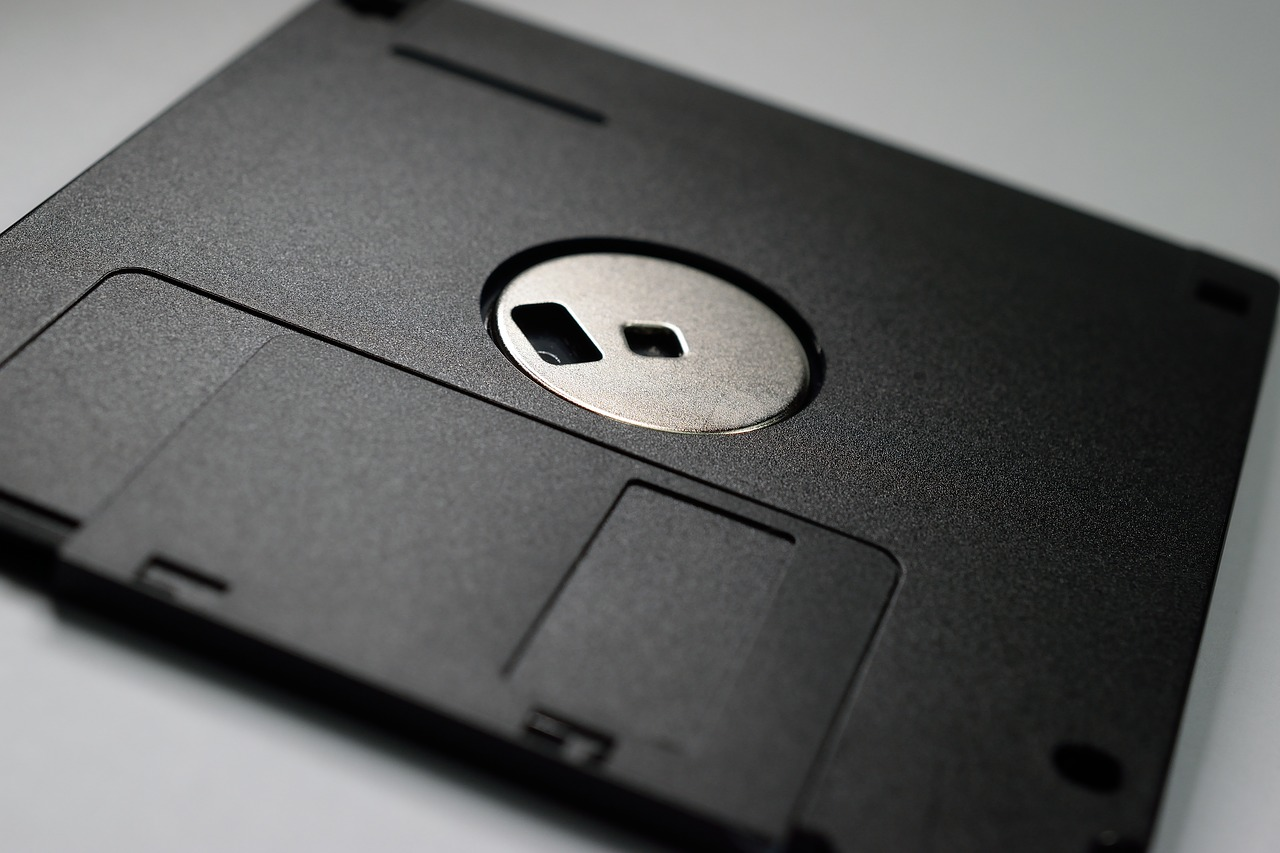
\includegraphics[width=0.25\textwidth]{img/computer-2346764_1280.jpg}
        \end{center}
      \end{figure}
      \bigskip
      Existem muitas variações disponíveis de passagens de Lorem Ipsum, mas a maioria sofreu algum tipo de alteração, seja por inserção de passagens com humor, ou palavras aleatórias que não parecem nem um pouco convincentes. Se você pretende usar uma passagem de Lorem Ipsum, precisa ter certeza de que não há algo embaraçoso escrito escondido no meio do texto. 
    \end{frame}
    
    
    \begin{frame}
      \frametitle{Métodos}
      \framesubtitle{Métodos, Técnicas e Tecnologias Utilizadas}      
        \begin{center}
            \begin{tabular}{ |c|c|p{7cm}| } 
            \hline
            Formula & Expressao & Descricao \\
            \hline
            \multirow{5}{*}{F1} & \multirow{5}{*}{$\sum_{n=1}^{\infty} 2^{-n}$} & \multirow{5}{7cm}{\footnotesize{Lorem Ipsum é simplesmente uma simulação de texto da indústria tipográfica e de impressos, e vem sendo utilizado desde o século XVI, quando um impressor desconhecido pegou uma bandeja de tipos e os embaralhou para fazer um livro de modelos de tipos.}~\cite{loremipsum}} \\ %linha1
            & & \\ %linha2
            & & \\ %linha3
            & & \\ %linha4
            & & \\ %linha5
            \hline
            \multirow{3}{*}{F2} & \multirow{3}{*}{$\sum_{n=1}^{\infty} 4^{-n}$} & \multirow{3}{7cm}{\footnotesize{Lorem Ipsum sobreviveu não só a cinco séculos, como também ao salto para a editoração eletrônica, permanecendo essencialmente inalterado.}~\cite{loremipsum}} \\ %linha1
            & & \\ %linha2
            & & \\ %linha3
            \hline
            \end{tabular}
        \end{center}
      
    \end{frame}
    
    %%%%%%%%%%%%%%%%%%%%%%%%%%%% ======== Desenvolvimento
    \section{Desenvolvimento}    
    \begin{frame}
      \frametitle{Desenvolvimento}
      \framesubtitle{Descrição do Problema}
      \begin{itemize}    
			\item Obtenção de um conjunto de dados de imagens para treinamento, validação e teste            
            \item Criação de variações da rede MobileNet.
            \item Realização do treinamento das redes criadas, utilizando transferência de conhecimento.
            \item Comparação entre as redes treinadas.
            \item Implementação do aplicativo e utilização do melhor modelo.
            \end{itemize}
    \end{frame}
    
    %%%%%%%%
    
    \begin{frame}
      \frametitle{Desenvolvimento}
      \framesubtitle{Atividades realizadas}      
      \begin{itemize}
        \item<1-> Levantamento das espécies de flores mais comuns nas redondezas do câmpus;\medskip
	    \item<2-> Obtenção do conjunto de dados:
	    		\begin{itemize}
	    			\item<3-> 16 classes;
	    			\item<4-> Google imagens e Oxford 102 Category Flower Dataset.
	    			\item<5-> Total de 4713 imagens: 70\% para treinamento, 10\% para validação e 20\% para teste. \medskip
	    		\end{itemize}
        \item<3-> Obtenção da rede MobileNet: 
        		\begin{itemize}
	    			\item<6-> Google AI Blog;
	    			\item<6-> Modelos já treinados com o conjunto de dados ImageNet; 
				\item<7-> Tamanho da imagem de entrada: 224x224x3;
				\item<7-> Tamanhos dos mapas de atributos das camadas de convolução: 25\%, 50\%, 75\% e 100\%.\medskip    		
	    		\end{itemize}     
      \end{itemize}
    \end{frame}
    
     \begin{frame}
      \frametitle{Desenvolvimento}
      \framesubtitle{Atividades realizadas}      
      \begin{itemize}
        \item<1-> Alterações realizadas: Modelo 1
        		 \begin{figure}[hbt]
      		 	\begin{center}
      				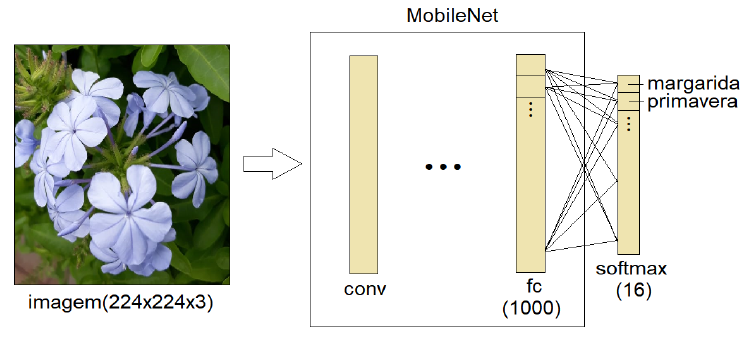
\includegraphics[width=0.8\textwidth]{img/model1.png}
      			\end{center}
      			\caption{Modelo 1~\cite{computer-1209641}}
      		\end{figure}
      \end{itemize}
    \end{frame}
    
    \begin{frame}
      \frametitle{Desenvolvimento}
      \framesubtitle{Atividades realizadas}      
      \begin{itemize}
        \item<1-> Alterações realizadas: Modelo 2
        		 \begin{figure}[hbt]
      		 	\begin{center}
      				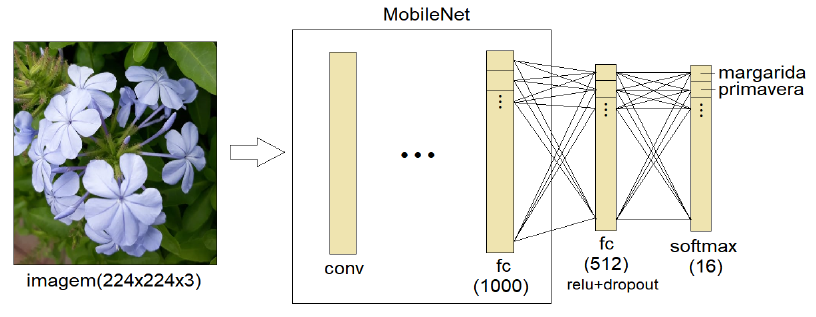
\includegraphics[height=0.35\textwidth]{img/model2.png}
      			\end{center}
      			\caption{Modelo 2~\cite{computer-1209641}}
      		\end{figure}
      \end{itemize}
    \end{frame}
    
    \begin{frame}
      \frametitle{Desenvolvimento}
      \framesubtitle{Atividades realizadas}      
      \begin{itemize}
        \item<1-> Resumo das alterações: \medskip
        \begin{figure}[hbt]
      		 	\begin{center}
      				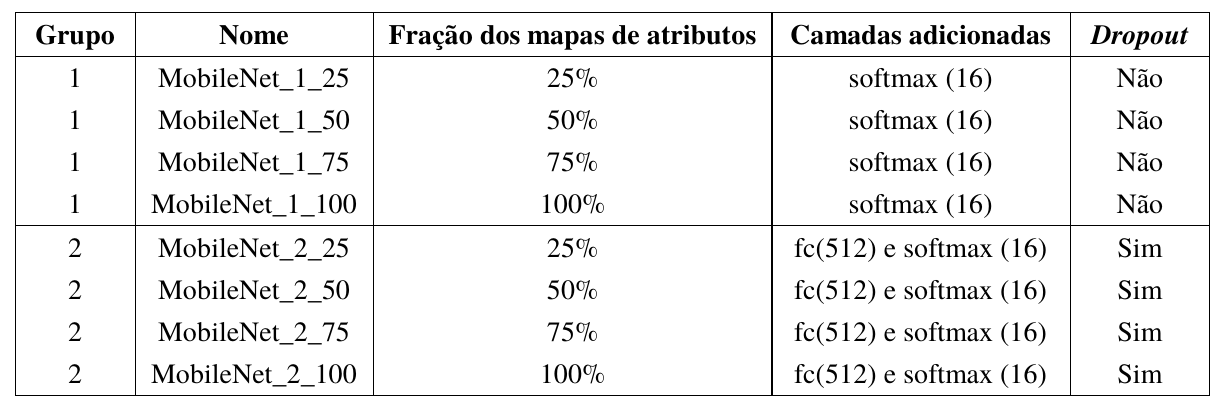
\includegraphics[height=.3 \textwidth]{img/models_table.png}
      			\end{center}
      			\caption{Resumos~\cite{computer-1209641}}
      		\end{figure}
      \end{itemize}
    \end{frame}
    
    \begin{frame}
      \frametitle{Desenvolvimento}
      \framesubtitle{Atividades realizadas}      
      \begin{itemize}
        \item<1-> Treinamento dos modelos propostos:
		 \begin{itemize}
        		\item<2-> Lotes de 100 imagens aleatórias;
        		\item<3-> 5000 iterações. \bigskip
		\end{itemize}        
        \item<4-> Implementação do aplicativo:
        \begin{itemize} 
        		\item<5-> Android Studio (Java);
        		\item<5-> TensorFlow para Android. \bigskip
        		   
		\end{itemize}
      \end{itemize}
    \end{frame}
        
    %%%%%%%%
    
    \begin{frame}
      \frametitle{Desenvolvimento}
      \framesubtitle{Resultados e Discussão}
      
      \only<1>{
        Objetivos \bigskip
        
        \begin{block}{Objetivos}
            \begin{itemize}
              \item Objetivo 1; \medskip
              \item Objetivo 2.
            \end{itemize}
        \end{block}
      }
    
    %%%%%%%%
    
      \only<2>{
          Para a validação foram utilizadas as fórmulas: \\ \medskip
          \scriptsize{
          Fórmula 1:
            \begin{equation}
            \overline{x} = \frac{1}{n} \ \sum_{i=1}^{n} x_i
            \end{equation}
          
          Fórmula 2:
            \begin{equation}
            \sigma_x = \sqrt{\frac{1}{n} \ \sum_{i=1}^{n} (x_i - \overline{x})^2 }
            \end{equation}
            }
      }
    
    \end{frame}
    
    %%%%%%%%%%%%%%%%%%%%%%%%%%%%
    \section{Conclusão}
    
    \begin{frame}
      \frametitle{Conclusão}
      \framesubtitle{Limitações \& Trabalhos Futuros}
      
      Limitações:
      \begin{itemize}
        \item Limitação 1;
        \item Limitação 2;
        \item Limitação 3.
      \end{itemize}
      
      \bigskip
      
      Trabalhos Futuros:
      \begin{itemize}
        \item Trabalhos Futuros 1~\cite{knuth-fa};
        \item Trabalhos Futuros 2.
      \end{itemize}
    \end{frame}
    
    %%%%%%%%
    
    \begin{frame}
      \frametitle{Conclusão}
      \framesubtitle{Contribuições}
        Contribuições\\
        Lorem Ipsum é um fato conhecido de todos que um leitor se distrairá com o conteúdo de texto legível de uma página quando estiver examinando sua diagramação.
        \cite{latexcompanion}.
        
        Agradecimentos ao ICMC~\cite{icmc}.
    \end{frame}
    
    %%%%%%%%%%%%%%%%%%%%%%%%%%%%
    \section{Referências}
    
    \begin{frame}[allowframebreaks]
      \frametitle{Referência Bibliográfica}
      \bibliographystyle{siam}
      
      \bibliography{referencias}
    \end{frame}
    
    %%%%%%%%%%%%%%%%%%%%%%%%%%%%
    
    \begin{frame}
        \frametitle{Obrigado!}
        \framesubtitle{Dúvidas?}
        \vskip -\baselineskip
        \vskip -0.55cm \hskip -0.55cm
        \begin{center}
          \maketitle
          \Large{\inserttitle} \\
          \insertauthor \\
          \footnotesize{\insertinstitute}
        \end{center}
    \end{frame}
    

\end{document}
